\chapter{Dataset}\label{chap:dataset}
In questo capitolo tratteremo la generazione del dataset posto alla base del modello che andremo a creare poi nel \autoref{chap:modello}, vederemo prima il dataset originale utilizzato e poi 
come è stato aumentato tramite l'utilizzo di ulteriori analizzatori statici per migliorarne la precisione delle rilevazioni, andando a ridurre il numero di falsi positivi.
Verrà poi presentato come le rilevazioni degli analizzatori statici sono utilizzate per la associazione fra un \textit{code snippet} e il relativo errore, poi come da quest'ultimo venga ricavato il codice in formato di \textit{ast context vector}.

\section{Dataset originale}
Come detto in precedenza questo dataset non è stato generato partendo da zero ma facendo riferimento al dataset creato da \cite{gelman2019source}. Il dataset consiste di circa 3000 progetti di GitHub, scritti in linguaggi C e \CPP,
 che rispettano due requisiti: hanno una licenza ridistribuibile e hanno almeno 10 stelle.
 Il secondo requisito ci serve per garantire che i progetti all'interno del dataset soddisfino dei requisiti di qualità, infatti come precedenti studi hanno mostrato (come ad esempio \cite{papamichail2016user}) si può utilizzare il numero
 di stelle su GitHub come un \textit{proxy} per la qualità del codice stesso.

Il dataset contiene per ogni progetto una serie di analisi effettuate: l'analisi di Doxygen che estrae le coppie codice-commento e l'analisi di Infer che produce un report di analisi statica degli errori.
Visto l'utilizzo che ne sarebbe stato fatto di questo dataset l'analisi di Doxygen è stata scartata. In \autoref{fig:dir_struct} si può vedere la struttura tipica di uno dei circa 3000 progetti presenti.
\begin{figure}
    \centering
    \scalebox{0.6}{
        \begin{forest}
            for tree={
                font=\ttfamily,
                grow'=0,
                child anchor=west,
                parent anchor=south,
                anchor=west,
                calign=first,
                inner xsep=7pt,
                edge path={
                  \noexpand\path [draw, \forestoption{edge}]
                  (!u.south west) +(7.5pt,0) |- (.child anchor) pic {folder} \forestoption{edge label};
                },
                % style for your file node 
                file/.style={edge path={\noexpand\path [draw, \forestoption{edge}]
                  (!u.south west) +(7.5pt,0) |- (.child anchor) \forestoption{edge label};},
                  inner xsep=2pt,font=\small\ttfamily
                             },
                before typesetting nodes={
                  if n=1
                    {insert before={[,phantom]}}
                    {}
                },
                fit=band,
                before computing xy={l=15pt},
              }  
        [Project-name
          [source
            [Project-name
                [Makefile, file]
                [File1.c, file]
                [File2.c, file]
                [..., file]
                [Folder1]
                [Folder2]
                [...]
            ]
          ]
          [derivatives
            [
                Infer-out
                [bugs.txt, file]
            ]
            ]
            [LICENSE, file]
            [url, file]
        ]
        \end{forest}
    }
    %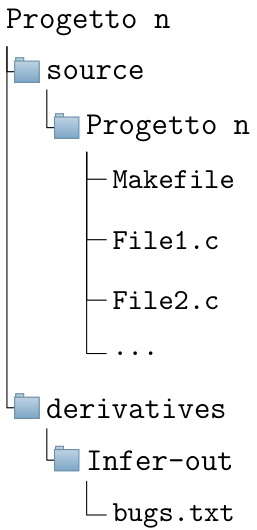
\includegraphics[scale=0.3]{images/immagineStrutturaDirectoryIniziale.png}
    \caption{La struttura della directory di un progetto del dataset iniziale}
    \label{fig:dir_struct}
\end{figure}

Come si può notare ogni progetto contiene anche un Makefile, elemento fondamentale perché gli analizzatori statici che andremo ad aggiungere spesso richiedono l'esistenza di un Makefile funzionante.

%Figura della struttura delle directory


%\subsection{Dataset originale}
 

%\subsection{Analizzatori utilizzati}

\section{Analizzatori di codice statici}
Un'analizzatore di codice è un programma che prende in input uno o più file e genera un report degli errori, cioè una lista di coppie del tipo $<$Errore, Posizione$>$. Di questi analizzatori ne esistono due macro categorie: statici e dinamici. 
Gli analizzatori statici sono programmi che effettuano controlli solo sul codice a livello testuale e che quindi non eseguono in nessuna maniera il codice, gli analizzatori dinamici sono invece analizzatori più complessi che effettuano controlli a \textit{run-time}
andando quindi ad'eseguire il codice stesso.

Gli analizzatori non sono però perfetti, infatti nell'insieme degli errori trovati si possono spesso trovare dei falsi positivi, cioè frammenti di codice segnati come erronei ma che in realtà non presentato nessun tipo di problema. Scopo appunto del dataset aumentato
è quello di ridurre il numero di falsi positivi.


\subsection{Analisi a livello di progetto}
La maggior parte degli analizzatori statici inoltre è in grado di lavorare a livello di progetti, andando quindi a risolvere correttamente gli \textit{include} (nel caso di C e \CPP), e quindi generando un output più significativo. 
Alcuni di questi per far ciò hanno bisogno di quello che viene chiamato \textit{compilation database} e, per soddisfare questo requisito, esistono strumenti appositi che utilizzano il Makefile per generarlo, nel caso di questo lavoro è stato utilizzato un programma
chiamato Bear


\subsection{Analizzatori ulteriori utilizzati}
Come analizzatori statici ulteriori da aggiungere in più a Infer, di cui ogni elemento del dataset ha già l'analisi sua associata, sono stati scelti i seguenti tre:
    \begin{itemize}
        \item L'analizzatore Cppcheck che, a detta degli autori, ha come scopo principale il ridurre il numero di falsi positivi.
        \item Il compilatore GCC che nonostante sia un compilatore vero e proprio ha anche funzionalità per l'analisi statica dei programmi attraverso la flag \textit{-fanalyzer}.
        \item Similarmente a GCC come terzo viene scelto il compilatore Clang che attraverso un suo tool chiamato Clang-Check è in grado di effettuare analisi statiche.
    \end{itemize}
Non sono invece stati usati analizzatori dinamici, questo perché il loro utilizzo in modo automatizzato è un operazione complicata se non quasi impossibile. 
Infatti quasi tutti i programmi prendono o dei parametri all'esecuzione o degli input durante l'esecuzione, ma fornire questi dati in modo consistente e sensato per il programma e in modo automatizzato rende il tutto veramente difficile.

L'utilizzo di essi però potrebbe portare a risultati molto interessanti poiché parte dei falsi positivi degli analizzatori statici deriva dal non poter decidere se frammenti di programmi sono o non sono eseguiti e quindi gli analizzano tutti, ma quello che può succedere
è che se in un frammento di programma che non viene sicuramente mai eseguito c'è un errore, l'analizzatore statico lo riferisce quello dinamico, correttamente, no.

%. La maggior parte degli analizzatori statici infatti


%\subsection{Fase 1: utilizzo di analizzatori statici per la generazione di report di errori}

%\subsection{Fase 2: aggregazione dei report}

%\subsbusection{Conversione degli errori}

%\subsection{Fase 3: }

%\subsection{Fase 4: generazione degli Ast Context}

%\section{Statistiche finali del dataset}